\documentclass[11pt]{article}
\usepackage[margin=1in]{geometry}
\usepackage{amsmath, amssymb}
\usepackage{graphicx}
\usepackage{booktabs}
\usepackage{hyperref}
\usepackage{float}
\usepackage{enumitem}
\usepackage{listings}
\usepackage{xcolor}

\lstset{
  language=R,
  basicstyle=\small\ttfamily,
  backgroundcolor=\color{gray!10},
  frame=single,
  breaklines=true,
  keywordstyle=\color{blue},
  commentstyle=\color{green!50!black},
  stringstyle=\color{red!70!black},
}

\setlength{\parindent}{0pt}
\setlength{\parskip}{6pt}

\title{\textbf{Homework 4 Solutions}\\Statistics 140}
\date{Due: April 8, 2026}
\author{}

\begin{document}
\maketitle

% =====================================================================
\section*{Problem 1}

\subsection*{Setup}

We load the \texttt{epigenetic.RData} dataset and fit the linear regression:
\[
  Y_i^{obs} = \beta_0 + \beta_1 W_i^{obs} + \epsilon_i,
\]
where $W_i^{obs} = 0$ for clean air and $W_i^{obs} = 1$ for ozone, and $\epsilon_i \sim N(0, \sigma^2)$.

\begin{lstlisting}
load("epigenetic.RData")
df <- epigenetic
model1 <- lm(cg09008103 ~ W, data = df)
summary(model1)
\end{lstlisting}

The data contains $N = 17$ participants: $N_0 = 7$ exposed to clean air and $N_1 = 10$ exposed to ozone.

\subsection*{Regression Coefficients}

\begin{align*}
  \hat{\beta}_0 &= 0.9701 \\
  \hat{\beta}_1 &= 0.0085 \\
  \hat{\sigma} &= 0.0024
\end{align*}

\textbf{Interpretation:}
\begin{itemize}
  \item $\hat{\beta}_0 = 0.9701$ is the estimated mean \textit{cg09008103} DNA methylation for the clean air group ($W_i = 0$).
  \item $\hat{\beta}_1 = 0.0085$ is the estimated difference in mean \textit{cg09008103} DNA methylation between the ozone group and the clean air group. Participants exposed to ozone have, on average, 0.0085 higher DNA methylation at this CpG site compared to those exposed to clean air.
\end{itemize}

\subsection*{Assumptions of the Regression Model}

The linear regression model assumes:
\begin{enumerate}
  \item \textbf{Linearity:} The relationship between the outcome and the treatment indicator is linear. Since $W_i$ is binary, this is automatically satisfied---the model simply compares two group means.
  \item \textbf{Independence:} The residuals $\epsilon_i$ are independent across participants.
  \item \textbf{Homoscedasticity:} The residuals have constant variance $\sigma^2$ across both groups. The sample variances are $s_{CA}^2 = 5.66 \times 10^{-6}$ and $s_{O_3}^2 = 6.18 \times 10^{-6}$, which are similar, so this assumption appears reasonable.
  \item \textbf{Normality:} The residuals are normally distributed. With only $N = 17$ observations, this assumption is difficult to verify and is particularly consequential for the validity of the asymptotic p-value.
\end{enumerate}

The regression model also implicitly assumes that the treatment indicator $W_i$ captures the full systematic variation, and that SUTVA holds (no interference between participants, no hidden versions of treatment).

\subsection*{Fisher-Exact Test}

We test the sharp null hypothesis:
\[
  H_0: Y_i(W_i = 0) = Y_i(W_i = 1) \quad \text{for all } i = 1, \ldots, 17.
\]

Under $H_0$, the observed outcomes are fixed: $Y_i^{obs} = Y_i(0) = Y_i(1)$ for all $i$. We use $\hat{\beta}_1$ as the test statistic and ``greater than'' as ``more extreme.''

The total number of possible randomizations is:
\[
  \binom{17}{10} = 19{,}448.
\]

Since this number is manageable, we enumerate all possible allocations exactly.

\begin{lstlisting}
combos <- combn(17, 10)
null_beta1 <- numeric(ncol(combos))
for (k in 1:ncol(combos)) {
  W_perm <- rep(0, 17)
  W_perm[combos[, k]] <- 1
  fit <- lm(Y ~ W_perm)
  null_beta1[k] <- coef(fit)[2]
}
fisher_pval <- mean(null_beta1 >= obs_beta1)
\end{lstlisting}

\begin{figure}[H]
  \centering
  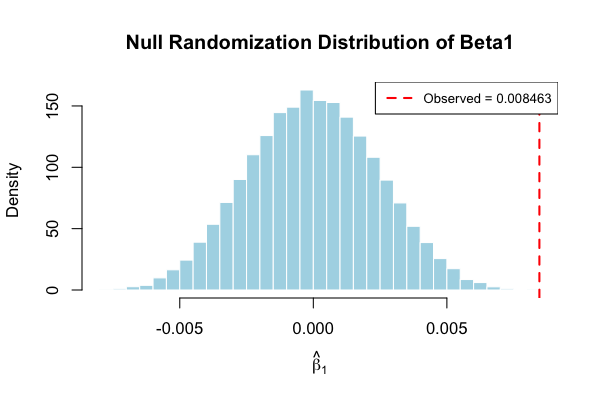
\includegraphics[width=0.75\textwidth]{null_beta1_histogram.png}
  \caption{Null randomization distribution of $\hat{\beta}_1$ under the sharp null. The red dashed line indicates the observed $\hat{\beta}_1 = 0.0085$.}
\end{figure}

The Fisher-exact p-value is:
\[
  p_{\text{Fisher}} = \frac{\#\{w \in \mathbb{W}^+: \hat{\beta}_1(w) \geq \hat{\beta}_1^{obs}\}}{19{,}448} \approx 0.0001.
\]

\textbf{What does the Fisher-exact p-value assume about the residuals?} The Fisher-exact p-value makes \textit{no distributional assumptions} about the residuals. Under the sharp null hypothesis, all potential outcomes are known (equal to the observed outcomes), and inference is derived purely from the randomization distribution---i.e., the known assignment mechanism. The residuals do not need to be normally distributed, homoscedastic, or independent in any model-based sense. The only source of randomness is the treatment assignment itself.

\textbf{Comparison of p-values:}
\begin{itemize}
  \item The Fisher-exact p-value (one-sided, greater than): $p_{\text{Fisher}} \approx 0.0001$.
  \item The asymptotic p-value from the regression model (one-sided): $p_{\text{asymp}} \approx 2.0 \times 10^{-6}$.
\end{itemize}

Both p-values provide strong evidence against the sharp null hypothesis, suggesting that ozone exposure is associated with increased \textit{cg09008103} DNA methylation. The asymptotic p-value is smaller because it relies on the additional assumptions of normality and homoscedasticity. The Fisher-exact p-value, being assumption-free (beyond SUTVA and the assignment mechanism), provides a more robust measure of evidence. Both lead to the same scientific conclusion: we find strong evidence that ozone exposure affects \textit{cg09008103} DNA methylation.

% =====================================================================
\newpage
\section*{Problem 2}

\subsection*{Group Counts}

We load the \texttt{epigenetic2.RData} dataset with 17 participants exposed to three conditions:

\begin{lstlisting}
load("epigenetic2.RData")
df2 <- epigenetic2
table(df2$Exposure)
\end{lstlisting}

\begin{center}
\begin{tabular}{lcc}
\toprule
Exposure & Code ($W_i$) & Count \\
\midrule
Clean Air (CA) & 0 & 5 \\
Diesel (D) & 1 & 6 \\
Ozone (O$_3$) & 2 & 6 \\
\bottomrule
\end{tabular}
\end{center}

\subsection*{Visualization}

\begin{lstlisting}
library(ggplot2)
ggplot(df2, aes(x = Exposure, y = cg09008103, fill = Exposure)) +
  geom_boxplot(alpha = 0.7) +
  geom_jitter(width = 0.1, size = 2) +
  theme_minimal() +
  labs(title = "cg09008103 DNA Methylation by Exposure Group",
       x = "Exposure", y = "cg09008103")
\end{lstlisting}

\begin{figure}[H]
  \centering
  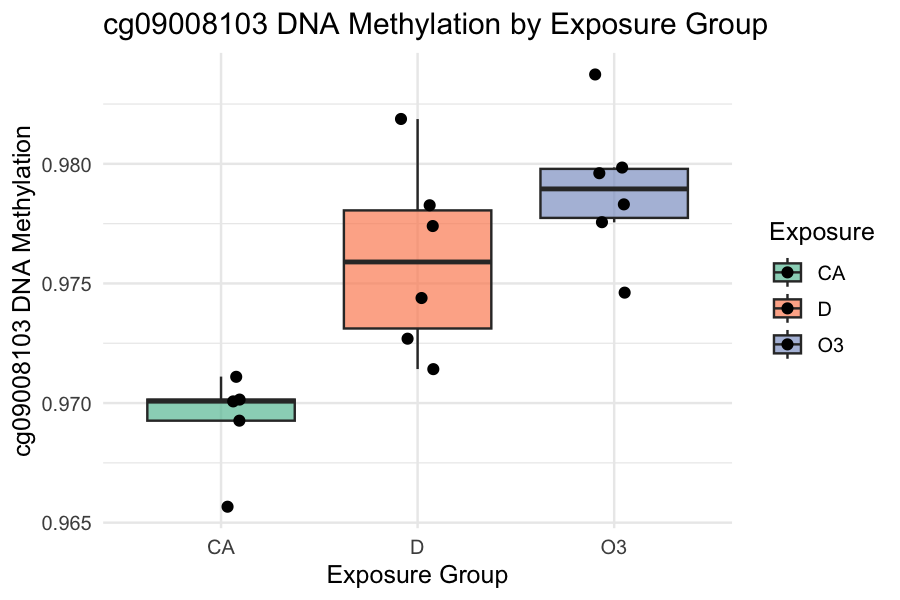
\includegraphics[width=0.7\textwidth]{boxplot_exposure.png}
  \caption{\textit{cg09008103} DNA methylation across the three exposure groups.}
\end{figure}

\textbf{Description:} The boxplot shows that the ozone group has the highest median \textit{cg09008103} DNA methylation, followed by the diesel group, with clean air having the lowest. The group means are:

\begin{center}
\begin{tabular}{lcc}
\toprule
Group & Mean & Variance \\
\midrule
Clean Air & 0.9693 & $4.45 \times 10^{-6}$ \\
Diesel & 0.9760 & $1.52 \times 10^{-5}$ \\
Ozone & 0.9789 & $9.09 \times 10^{-6}$ \\
\bottomrule
\end{tabular}
\end{center}

The variances differ across groups---Diesel has the largest variance ($1.52 \times 10^{-5}$), about 3.4 times larger than Clean Air ($4.45 \times 10^{-6}$). This suggests potential heteroscedasticity, which is a concern for the standard ANOVA and regression assumptions.

\subsection*{ANOVA}

\begin{lstlisting}
anova_model <- aov(cg09008103 ~ Exposure, data = df2)
summary(anova_model)
\end{lstlisting}

\begin{center}
\begin{tabular}{lccccc}
\toprule
 & Df & Sum Sq & Mean Sq & F value & Pr($>$F) \\
\midrule
Exposure & 2 & $2.646 \times 10^{-4}$ & $1.323 \times 10^{-4}$ & 13.29 & 0.00058 \\
Residuals & 14 & $1.393 \times 10^{-4}$ & $9.950 \times 10^{-6}$ & & \\
\bottomrule
\end{tabular}
\end{center}

The F statistic is:
\[
  F = \frac{\text{MSB}}{\text{MSW}} = \frac{1.323 \times 10^{-4}}{9.950 \times 10^{-6}} = 13.29.
\]

\textbf{Interpretation of the F statistic:} The F statistic is the ratio of the between-group mean square (MSB) to the within-group mean square (MSW). MSB measures the variability of the group means around the overall mean, while MSW measures the variability of observations within each group. A large $F$ indicates that the between-group variability is much larger than what would be expected from within-group variability alone, providing evidence that at least one group mean differs from the others.

\subsection*{Regression Analysis}

\begin{lstlisting}
df2$Exposure <- relevel(factor(df2$Exposure), ref = "CA")
reg_model <- lm(cg09008103 ~ Exposure, data = df2)
summary(reg_model)
\end{lstlisting}

With clean air as the reference category:
\begin{align*}
  \hat{\beta}_0 &= 0.9693 \quad (\text{mean for clean air}) \\
  \hat{\beta}_{\text{Diesel}} &= 0.0068 \quad (p = 0.003) \\
  \hat{\beta}_{\text{Ozone}} &= 0.0097 \quad (p = 0.0002)
\end{align*}

Both diesel and ozone are associated with significantly higher \textit{cg09008103} DNA methylation compared to clean air based on the asymptotic p-values from the regression model.

\textbf{Issues with these additional tests:}
\begin{enumerate}
  \item \textbf{Multiple comparisons:} Performing pairwise comparisons after ANOVA without adjusting for multiplicity inflates the family-wise error rate. With two pairwise tests (ozone vs.\ clean air and diesel vs.\ clean air), we increase the probability of at least one false positive.
  \item \textbf{Post-hoc testing:} These pairwise comparisons are conducted after observing that the global F test is significant. Without a pre-specified plan, this can be considered data dredging.
  \item \textbf{Asymptotic assumptions:} The regression p-values rely on normality and homoscedasticity assumptions. With only 5--6 observations per group and unequal variances, these asymptotic approximations may not be reliable.
\end{enumerate}

\subsection*{Number of Randomizations}

The number of ways to randomize 17 participants into 5 clean air, 6 diesel, and 6 ozone is given by the multinomial coefficient:
\[
  \binom{17}{5, 6, 6} = \frac{17!}{5! \cdot 6! \cdot 6!} = 5{,}717{,}712.
\]

\subsection*{Fisherian Inference for the Global Sharp Null}

\textbf{Potential outcome notation.} Let $Y_i(W_i = 0)$, $Y_i(W_i = 1)$, and $Y_i(W_i = 2)$ denote the potential outcomes of participant $i$ under clean air, diesel, and ozone, respectively. The global sharp null hypothesis states:
\[
  H_0: Y_i(W_i = 0) = Y_i(W_i = 1) = Y_i(W_i = 2) \quad \text{for all } i = 1, \ldots, 17.
\]

Under $H_0$, all potential outcomes equal the observed values: $Y_i(0) = Y_i(1) = Y_i(2) = Y_i^{obs}$ for all $i$. This makes $H_0$ sharp because all missing potential outcomes are known, and we can compute the test statistic for any possible allocation.

We use the F statistic from the ANOVA as the test statistic and ``greater than'' for ``more extreme.'' We justify this choice because:
\begin{itemize}
  \item The F statistic is a natural omnibus test statistic for comparing multiple group means simultaneously.
  \item It is sensitive to differences in any direction among the three groups.
  \item Using ``greater than'' is appropriate because the F statistic is one-sided by construction---larger values indicate more evidence against the null of equal group means.
\end{itemize}

Since the total number of randomizations ($5{,}717{,}712$) is large, we approximate the null randomization distribution using 100,000 Monte Carlo randomized allocations with seed 2026.

\begin{lstlisting}
set.seed(2026)
n_perm <- 100000
null_f <- numeric(n_perm)
for (k in 1:n_perm) {
  W_perm <- sample(W2_obs)  # permute observed assignments
  df_perm <- data.frame(Y = Y2, W = factor(W_perm))
  anova_perm <- aov(Y ~ W, data = df_perm)
  null_f[k] <- summary(anova_perm)[[1]]$"F value"[1]
}
fisher_pval <- mean(null_f >= f_stat)
\end{lstlisting}

\begin{figure}[H]
  \centering
  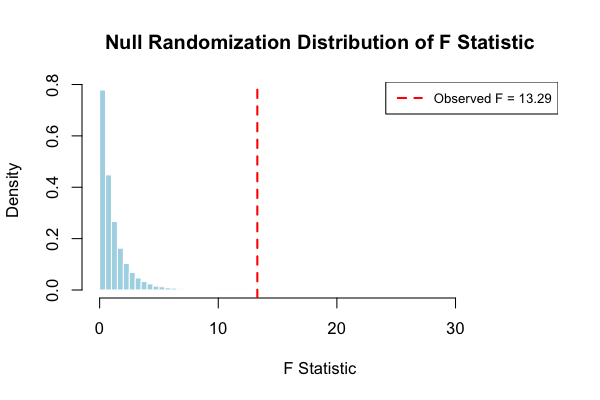
\includegraphics[width=0.75\textwidth]{null_f_histogram.png}
  \caption{Null randomization distribution of the F statistic. The observed $F = 13.29$ (red dashed line) falls far in the right tail.}
\end{figure}

The approximated Fisherian p-value is:
\[
  p_{\text{Fisher}} = \frac{\#\{r: F^{(r)} \geq F^{obs}\}}{100{,}000} \approx 0.0009.
\]

\textbf{Interpretation:} The p-value of 0.0009 provides strong evidence against the global sharp null hypothesis. Under the assumption that exposure has no effect on any participant's \textit{cg09008103} DNA methylation, observing an F statistic as extreme as 13.29 would occur with probability approximately 0.001. This is highly unusual, suggesting that at least one exposure group has a different effect on DNA methylation.

\textbf{Decision: Continue to further assess group differences.} Since we reject the global sharp null, it is scientifically appropriate to investigate which specific exposure comparisons drive this effect. However, we should be mindful of the multiple comparisons issue.

\subsection*{Pairwise Fisherian Inference}

We conduct pairwise Fisher randomization tests for:
\begin{enumerate}
  \item \textbf{Ozone vs.\ Clean Air}: Using the difference in means as the test statistic and ``greater than'' as more extreme.

  Observed difference: $\bar{Y}_{O_3} - \bar{Y}_{CA} = 0.0097$.

  Approximated Fisher p-value (100,000 permutations, seed 2026): $p \approx 0.002$.

  \item \textbf{Diesel vs.\ Clean Air}: Using the difference in means as the test statistic and ``greater than'' as more extreme.

  Observed difference: $\bar{Y}_{D} - \bar{Y}_{CA} = 0.0068$.

  Approximated Fisher p-value (100,000 permutations, seed 2026): $p \approx 0.002$.
\end{enumerate}

\textbf{Issues with pairwise tests:}
\begin{itemize}
  \item \textbf{Multiple comparisons:} Conducting two pairwise tests inflates the overall Type I error rate. A Bonferroni correction could be applied (multiply p-values by 2), but even after correction, both adjusted p-values ($\approx 0.004$) remain small.
  \item \textbf{Subset randomization:} The pairwise Fisherian tests condition on the subset of units in the two groups being compared, which changes the randomization distribution. The original experiment randomized across three groups, not two.
\end{itemize}

\textbf{Comparison of Fisherian and Asymptotic Inference:}

\begin{center}
\begin{tabular}{lccc}
\toprule
Comparison & Fisher p-value & Asymptotic p-value & Comment \\
\midrule
Global (F test) & 0.0009 & 0.00058 & Both strongly significant \\
Ozone vs.\ CA & 0.002 & 0.0002 & Fisher is more conservative \\
Diesel vs.\ CA & 0.002 & 0.003 & Similar magnitude \\
\bottomrule
\end{tabular}
\end{center}

The Fisherian p-values are generally comparable to, but slightly larger than, the asymptotic p-values. This is expected because:
\begin{itemize}
  \item The asymptotic p-values rely on distributional assumptions (normality, homoscedasticity) that may not hold perfectly with such small samples.
  \item The Fisherian p-values are exact (conditional on the observed outcomes) and make no distributional assumptions beyond the assignment mechanism.
  \item Both approaches lead to the same qualitative conclusion: there is strong evidence that both ozone and diesel exposure affect \textit{cg09008103} DNA methylation compared to clean air.
\end{itemize}

% =====================================================================
\newpage
\section*{Problem 3}

\subsection*{Setup}

In a crossover randomized experiment, each participant $i$ is observed in two periods $j \in \{1, 2\}$. In period 1, participant $i$ receives treatment $W_{i,1}$, and in period 2, they receive the opposite treatment $W_{i,2} = 1 - W_{i,1}$. The potential outcome $Y_{i,j}(W_{i,j} = w_{i,j})$ denotes participant $i$'s outcome at period $j$ under treatment $w_{i,j}$. The causal estimand is:
\[
  \tau = \frac{1}{N} \sum_{i=1}^{N} \frac{1}{2} \Big[ \big(Y_{i,1}(W_{i,1}=1) - Y_{i,1}(W_{i,1}=0)\big) + \big(Y_{i,2}(W_{i,2}=1) - Y_{i,2}(W_{i,2}=0)\big) \Big],
\]
which is the period- and population-average causal effect of treatment versus control.

\subsection*{Sharp Null Hypothesis}

The sharp null hypothesis associated with the period- and population-average causal effect $\tau$ states:
\[
  H_0: Y_{i,j}(W_{i,j} = 1) = Y_{i,j}(W_{i,j} = 0) \quad \text{for all } i = 1, \ldots, N \text{ and all } j = 1, 2.
\]

In words: for \textit{every} participant $i$ and \textit{every} period $j$, the potential outcome under treatment equals the potential outcome under control. This is a sharp null because it specifies every individual's treatment effect to be exactly zero in every period, thereby allowing us to fill in all missing potential outcomes: $Y_{i,j}(1) = Y_{i,j}(0) = Y_{i,j}^{obs}$ for all $i$ and $j$.

\subsection*{Alternative Test Statistic to $T_{paired}$}

The standard paired test statistic is:
\[
  T_{paired} = \frac{1}{N} \sum_{i=1}^{N} (2W_{i,1} - 1)\left(Y_{i,1}^{obs} - Y_{i,2}^{obs}\right),
\]
which computes the average of the within-participant differences, signed by the treatment assignment.

An alternative test statistic is the \textbf{Wilcoxon signed-rank statistic}. Let $D_i = (2W_{i,1} - 1)(Y_{i,1}^{obs} - Y_{i,2}^{obs})$ be the signed within-participant difference. The Wilcoxon signed-rank statistic is:
\[
  T_{WSR} = \sum_{i=1}^{N} \text{rank}(|D_i|) \cdot \text{sign}(D_i).
\]

This statistic ranks the absolute values of the paired differences and sums the ranks with the sign of each difference. It is more robust to outliers than $T_{paired}$ because it is based on ranks rather than the actual magnitudes of the differences. Under the sharp null, the distribution of $T_{WSR}$ can be derived from the randomization distribution, since each participant's assignment $W_{i,1} \in \{0, 1\}$ is equally likely, and under $H_0$, flipping the assignment does not change the outcome.

% =====================================================================
\newpage
\section*{Problem 4}

\subsection*{Setup}

We consider a randomized experiment with $N$ participants stratified by sex: $N(m)$ males and $N(f)$ females, with $N = N(m) + N(f)$. Within each stratum, a completely randomized design is implemented. Let $Y_i(W_i = 0)$ and $Y_i(W_i = 1)$ denote participant $i$'s potential outcomes under control and treatment.

\subsection*{Average Causal Effect}

The population-average causal effect is:
\[
  \tau = \frac{1}{N} \sum_{i=1}^{N} \left[Y_i(1) - Y_i(0)\right].
\]

We can decompose this into stratum-specific effects. Let $\tau(m)$ and $\tau(f)$ denote the average treatment effects for males and females:
\[
  \tau(m) = \frac{1}{N(m)} \sum_{i \in \text{males}} \left[Y_i(1) - Y_i(0)\right], \quad
  \tau(f) = \frac{1}{N(f)} \sum_{i \in \text{females}} \left[Y_i(1) - Y_i(0)\right].
\]

Then:
\[
  \boxed{\tau = \frac{N(m)}{N} \cdot \tau(m) + \frac{N(f)}{N} \cdot \tau(f).}
\]

This is a weighted average of the stratum-specific treatment effects, weighted by the stratum sizes.

\subsection*{Estimator for $\tau$}

Within each stratum $s \in \{m, f\}$, let $N_t(s)$ and $N_c(s)$ denote the number of treated and control units. The difference-in-means estimator within stratum $s$ is:
\[
  \hat{\tau}(s) = \bar{Y}_t^{obs}(s) - \bar{Y}_c^{obs}(s) = \frac{1}{N_t(s)} \sum_{\substack{i \in s \\ W_i = 1}} Y_i^{obs} - \frac{1}{N_c(s)} \sum_{\substack{i \in s \\ W_i = 0}} Y_i^{obs}.
\]

The estimator for $\tau$ mirrors the population decomposition:
\[
  \boxed{\hat{\tau} = \frac{N(m)}{N} \cdot \hat{\tau}(m) + \frac{N(f)}{N} \cdot \hat{\tau}(f).}
\]

\subsection*{Sampling Variance of $\hat{\tau}$}

Since randomization is conducted independently within each stratum (the defining feature of stratified randomization), $\hat{\tau}(m)$ and $\hat{\tau}(f)$ are \textit{independent}. Therefore:
\[
  \text{Var}(\hat{\tau}) = \left(\frac{N(m)}{N}\right)^2 \text{Var}(\hat{\tau}(m)) + \left(\frac{N(f)}{N}\right)^2 \text{Var}(\hat{\tau}(f)).
\]

Within each stratum $s \in \{m, f\}$, the variance of the difference-in-means estimator under a completely randomized design is (Neyman, 1923):
\[
  \text{Var}(\hat{\tau}(s)) = \frac{S^2_s(1)}{N_t(s)} + \frac{S^2_s(0)}{N_c(s)} - \frac{S^2_s(\tau)}{N(s)},
\]
where $S^2_s(1)$, $S^2_s(0)$ are the finite-population variances of the potential outcomes under treatment and control within stratum $s$, and $S^2_s(\tau)$ is the variance of the individual treatment effects within stratum $s$.

Thus:
\[
  \boxed{\text{Var}(\hat{\tau}) = \left(\frac{N(m)}{N}\right)^2 \left[\frac{S^2_m(1)}{N_t(m)} + \frac{S^2_m(0)}{N_c(m)} - \frac{S^2_m(\tau)}{N(m)}\right] + \left(\frac{N(f)}{N}\right)^2 \left[\frac{S^2_f(1)}{N_t(f)} + \frac{S^2_f(0)}{N_c(f)} - \frac{S^2_f(\tau)}{N(f)}\right].}
\]

\textbf{Explanation:}
\begin{itemize}
  \item The overall variance decomposes into two independent stratum-level contributions because the stratified design ensures that randomization within the male stratum is independent of randomization within the female stratum.
  \item Each stratum's contribution is weighted by the squared proportion $\left(\frac{N(s)}{N}\right)^2$, reflecting the fact that $\hat{\tau}$ is a weighted average with weights $N(s)/N$.
  \item Within each stratum, the variance formula is the standard Neyman variance for a CRD. The term $-S^2_s(\tau)/N(s)$ reflects that heterogeneous treatment effects within a stratum actually reduce the variance of the estimator.
  \item Stratification is generally beneficial: by conducting randomization within homogeneous subgroups, we reduce the within-stratum variability, leading to a more precise estimate of $\tau$ compared to a completely randomized design without stratification.
\end{itemize}

% =====================================================================
\newpage
\section*{Problem 5}

\subsection*{Two-Factor Experiment}

Consider a two-factor experiment where factor $A$ has levels $\{-1, +1\}$ and factor $B$ has levels $\{-1, +1\}$. There are $2^2 = 4$ treatment combinations.

\textbf{Science Table:}

The science table lists all potential outcomes for each unit $i$ under all treatment combinations:

\begin{center}
\begin{tabular}{c|cccc}
\toprule
Unit $i$ & $Y_i(A=-1, B=-1)$ & $Y_i(A=-1, B=+1)$ & $Y_i(A=+1, B=-1)$ & $Y_i(A=+1, B=+1)$ \\
\midrule
1 & $Y_1(-1,-1)$ & $Y_1(-1,+1)$ & $Y_1(+1,-1)$ & $Y_1(+1,+1)$ \\
2 & $Y_2(-1,-1)$ & $Y_2(-1,+1)$ & $Y_2(+1,-1)$ & $Y_2(+1,+1)$ \\
$\vdots$ & $\vdots$ & $\vdots$ & $\vdots$ & $\vdots$ \\
$N$ & $Y_N(-1,-1)$ & $Y_N(-1,+1)$ & $Y_N(+1,-1)$ & $Y_N(+1,+1)$ \\
\bottomrule
\end{tabular}
\end{center}

Each row contains $2^2 = 4$ potential outcomes for each unit---one for each treatment combination. Due to the Fundamental Problem of Causal Inference, only one of the four potential outcomes per unit is observed.

\textbf{Observed Table:}

\begin{center}
\begin{tabular}{c|cc|cccc}
\toprule
Unit $i$ & $A_i^{obs}$ & $B_i^{obs}$ & $Y_i(-1,-1)$ & $Y_i(-1,+1)$ & $Y_i(+1,-1)$ & $Y_i(+1,+1)$ \\
\midrule
1 & $-1$ & $-1$ & $Y_1^{obs}$ & ? & ? & ? \\
2 & $-1$ & $+1$ & ? & $Y_2^{obs}$ & ? & ? \\
$\vdots$ & $\vdots$ & $\vdots$ & & & & \\
$N$ & $+1$ & $+1$ & ? & ? & ? & $Y_N^{obs}$ \\
\bottomrule
\end{tabular}
\end{center}

Only the potential outcome corresponding to the assigned treatment combination is observed for each unit; all other entries are missing (denoted by ``?'').

\subsection*{Three-Factor Experiment}

With three factors $A$, $B$, and $C$, each having two levels $\{-1, +1\}$, there are now $2^3 = 8$ treatment combinations. The science table would have $N$ rows (one per unit) and $8$ columns of potential outcomes---one for each treatment combination.

\textbf{Treatment combinations in lexicographic order:}

\begin{center}
\begin{tabular}{c|ccc}
\toprule
Combination & $A$ & $B$ & $C$ \\
\midrule
1 & $-1$ & $-1$ & $-1$ \\
2 & $-1$ & $-1$ & $+1$ \\
3 & $-1$ & $+1$ & $-1$ \\
4 & $-1$ & $+1$ & $+1$ \\
5 & $+1$ & $-1$ & $-1$ \\
6 & $+1$ & $-1$ & $+1$ \\
7 & $+1$ & $+1$ & $-1$ \\
8 & $+1$ & $+1$ & $+1$ \\
\bottomrule
\end{tabular}
\end{center}

\textbf{Science Table} (for three factors):

\begin{center}
\small
\begin{tabular}{c|cccccccc}
\toprule
$i$ & $Y_i(-1,-1,-1)$ & $Y_i(-1,-1,+1)$ & $Y_i(-1,+1,-1)$ & $Y_i(-1,+1,+1)$ & $Y_i(+1,-1,-1)$ & $Y_i(+1,-1,+1)$ & $Y_i(+1,+1,-1)$ & $Y_i(+1,+1,+1)$ \\
\midrule
1 & $Y_1$ & $Y_1$ & $Y_1$ & $Y_1$ & $Y_1$ & $Y_1$ & $Y_1$ & $Y_1$ \\
$\vdots$ & $\vdots$ & $\vdots$ & $\vdots$ & $\vdots$ & $\vdots$ & $\vdots$ & $\vdots$ & $\vdots$ \\
$N$ & $Y_N$ & $Y_N$ & $Y_N$ & $Y_N$ & $Y_N$ & $Y_N$ & $Y_N$ & $Y_N$ \\
\bottomrule
\end{tabular}
\end{center}

\textbf{What changes with three factors:}
\begin{itemize}
  \item The science table expands from 4 columns of potential outcomes to 8 columns---one for each of the $2^3 = 8$ treatment combinations.
  \item The observed table similarly has 8 potential outcome columns, but for each unit, only 1 of the 8 is observed (the one matching the assigned combination), and the other 7 are missing.
  \item The number of causal estimands increases: beyond the three main effects ($A$, $B$, $C$), there are three two-way interactions ($AB$, $AC$, $BC$) and one three-way interaction ($ABC$), for a total of 7 factorial effects.
  \item The assignment mechanism now assigns each unit to one of 8 treatment combinations, rather than one of 4.
\end{itemize}

\end{document}
